\documentclass[aspectratio=169]{beamer}

% Theme selection
\usetheme{Madrid}
\usecolortheme{whale}

% Packages
\usepackage{graphicx}
\usepackage{tikz}
\usetikzlibrary{shapes,arrows,positioning}
\usepackage{booktabs}
\usepackage{listings}
\usepackage{xcolor}
\usepackage{CJKutf8}

% Custom colors
\definecolor{codegreen}{rgb}{0,0.6,0}
\definecolor{codegray}{rgb}{0.5,0.5,0.5}
\definecolor{codepurple}{rgb}{0.58,0,0.82}
\definecolor{backcolour}{rgb}{0.95,0.95,0.92}

% Code listing style
\lstdefinestyle{mystyle}{
    backgroundcolor=\color{backcolour},   
    commentstyle=\color{codegreen},
    keywordstyle=\color{magenta},
    numberstyle=\tiny\color{codegray},
    stringstyle=\color{codepurple},
    basicstyle=\ttfamily\footnotesize,
    breakatwhitespace=false,         
    breaklines=true,                 
    captionpos=b,                    
    keepspaces=true,                 
    numbers=left,                    
    numbersep=5pt,                  
    showspaces=false,                
    showstringspaces=false,
    showtabs=false,                  
    tabsize=2
}
\lstset{style=mystyle}

\begin{document}
\begin{CJK*}{UTF8}{gbsn}

% Title Info
\title[Tarkov Weapon Optimizer]{Tarkov Weapon Mod Optimizer}
\subtitle{Automated Build Optimization using Constraint Programming}
\author{Imposs1ble嗨}
\date{\today}

\begin{frame}
    \titlepage
\end{frame}

% Section 1: Introduction
\section{Introduction}

% Slide 3: The Problem
\begin{frame}{The Problem: Complexity in Escape from Tarkov}
    \textit{Escape from Tarkov} features one of the most complex weapon modification systems in gaming.

    \vspace{0.3cm}
    \textbf{Challenges for New Players:}
    \begin{itemize}
        \item \textbf{Overwhelming scale:} 2,500+ mods, each affecting recoil, ergonomics, weight, accuracy
        \item \textbf{Nested compatibility:} Mods attach to mods (rail $\to$ mount $\to$ sight)
        \item \textbf{Combinatorial explosion:} A single AR-15 has 50+ slots, millions of valid builds
        \item \textbf{Non-obvious trade-offs:} Is a 50k grip worth it over a 5k one?
        \item \textbf{Dynamic availability:} Prices change; items locked behind trader levels, quests, and flea market access
    \end{itemize}

    \vspace{0.3cm}
    \textbf{Result:} Players spend hours theory-crafting or blindly copy ``meta builds'' without understanding trade-offs.
\end{frame}

% Slide 4: The Solution
\begin{frame}{The Solution: Automated Optimization}
    \textbf{Project Goal:}
    Create a tool that mathematically guarantees the "best" weapon build for a given set of constraints.

    \vspace{0.4cm}
    \begin{columns}
        \column{0.5\textwidth}
        \textbf{Use Cases:}
        \begin{itemize}
            \item \textit{"I have 200k roubles---what's the best M4 I can build?"}
            \item \textit{"What's the absolute lowest recoil AK, money no object?"}
            \item \textit{"I'm level 15 with LL2 traders---what can I actually buy?"}
            \item \textit{"Is spending 100k more actually worth it?"}
            \item \textit{"Show me all viable builds on a budget curve"}
        \end{itemize}

        \column{0.5\textwidth}
        \textbf{Key Capabilities:}
        \begin{itemize}
            \item \textbf{Multi-objective}: Balance recoil, ergonomics, and price
            \item \textbf{Budget-aware}: Hard limit or soft penalty on cost
            \item \textbf{Trader filtering}: Respect loyalty levels (LL1--LL4)
            \item \textbf{Flea market toggle}: Include or exclude market prices
            \item \textbf{Pareto frontier}: Visualize price vs. performance trade-offs
        \end{itemize}
    \end{columns}
\end{frame}

% Section 2: Architecture
\section{System Architecture}

% Slide: Pipeline Overview
\begin{frame}{Pipeline Overview}
    \begin{center}
    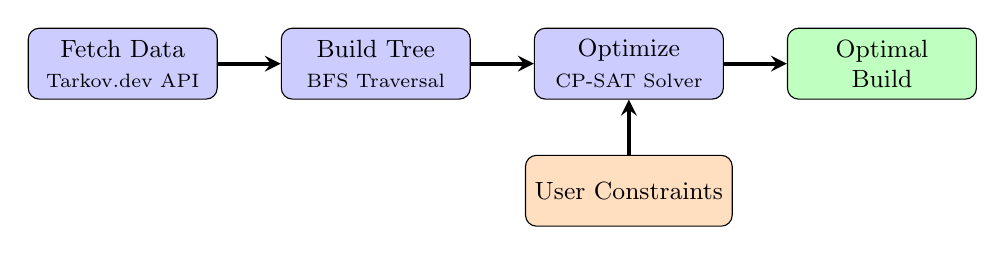
\begin{tikzpicture}[
        node distance=0.8cm,
        every node/.style={font=\small},
        box/.style={draw, rectangle, rounded corners, fill=blue!20, minimum width=2.4cm, minimum height=0.9cm, align=center},
        arrow/.style={->, thick, >=stealth, line width=1.5pt}
    ]
        % Main pipeline - horizontal
        \node[box] (fetch) {Fetch Data\\{\scriptsize Tarkov.dev API}};
        \node[box, right=of fetch] (compat) {Build Tree\\{\scriptsize BFS Traversal}};
        \node[box, right=of compat] (solve) {Optimize\\{\scriptsize CP-SAT Solver}};
        \node[box, right=of solve, fill=green!25] (result) {Optimal\\Build};

        % User input from below
        \node[box, below=0.7cm of solve, fill=orange!25] (user) {User Constraints};

        % Arrows
        \draw[arrow] (fetch) -- (compat);
        \draw[arrow] (compat) -- (solve);
        \draw[arrow] (solve) -- (result);
        \draw[arrow] (user) -- (solve);
    \end{tikzpicture}
    \end{center}
\end{frame}

% Slide 5: Fetching Data
\begin{frame}{Fetching Data}
    \begin{columns}
        \column{0.45\textwidth}
        \textbf{Tarkov.dev GraphQL API}

        \vspace{0.3cm}
        \begin{itemize}
            \item Queries all guns, mods, and compatibility rules
            \item \textbf{Up-to-date prices} from traders and flea market
            \item Trader loyalty level requirements
            \item Real-time flea market prices
            \item Local caching for speed
        \end{itemize}

        \column{0.55\textwidth}
        \begin{center}
            \includegraphics[width=\textwidth]{imgs/tarkov_dev.jpg}
        \end{center}
    \end{columns}
\end{frame}

% Slide 6a: Data Processing Pipeline
% \begin{frame}{Data Processing: From API to Item Lookup}
%     \textbf{Step 1: Raw API Data Normalization}

%     \vspace{0.2cm}
%     \begin{columns}
%         \column{0.5\textwidth}
%         \textbf{Slot Extraction Challenges:}
%         \begin{itemize}
%             \item Guns and mods have different property structures
%             \item \texttt{filters.allowedItems} can be:
%             \begin{itemize}
%                 \item List of objects: \texttt{[\{"id": "abc"\}]}
%                 \item List of strings: \texttt{["abc", "def"]}
%             \end{itemize}
%             \item Must normalize to flat list of IDs
%         \end{itemize}

%         \vspace{0.3cm}
%         \textbf{Price Validation:}
%         \begin{itemize}
%             \item Mods without valid \texttt{buyFor} offers are filtered out
%             \item Prevents selecting items that can't actually be purchased
%         \end{itemize}

%         \column{0.5\textwidth}
%         \textbf{Stat Normalization:}
%         \begin{itemize}
%             \item \textbf{Recoil modifier} formats differ:
%             \begin{itemize}
%                 \item Top-level: integer \% (e.g., \texttt{-5})
%                 \item Properties: decimal (e.g., \texttt{-0.05})
%             \end{itemize}
%             \item Normalize all to decimal format
%             \item Handle null/missing values gracefully
%         \end{itemize}

%         \vspace{0.3cm}
%         \textbf{Conflict Extraction:}
%         \begin{itemize}
%             \item \texttt{conflictingItems}: Items that can't coexist
%             \item \texttt{conflictingSlotIds}: Slots blocked by this item
%         \end{itemize}
%     \end{columns}
% \end{frame}

% Slide 6c: BFS Compatibility Tree
\begin{frame}{Building the Compatibility Tree}
    \begin{columns}
        \column{0.55\textwidth}
        \textbf{BFS Process:}
        \begin{enumerate}
            \item Start from the base weapon's slots
            \item For each slot, find all allowed items
            \item Add those items to the queue
            \item For each item, discover \textit{its} slots
            \item Repeat until no new items found
        \end{enumerate}

        \vspace{0.2cm}
        \textbf{Data Structures Built:}
        \begin{itemize}
            \item \texttt{slot\_items}: Slot $\to$ [compatible items]
            \item \texttt{slot\_owner}: Slot $\to$ parent item
            \item \texttt{item\_to\_slots}: Item $\to$ [owned slots]
        \end{itemize}

        \column{0.45\textwidth}
        \begin{center}
        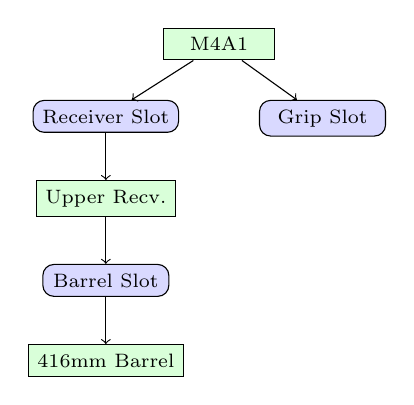
\begin{tikzpicture}[
            node distance=0.6cm,
            every node/.style={font=\scriptsize},
            slot/.style={draw, rectangle, rounded corners, fill=blue!15, minimum width=1.6cm, minimum height=0.4cm},
            item/.style={draw, rectangle, fill=green!15, minimum width=1.4cm, minimum height=0.4cm}
        ]
            \node[item] (gun) {M4A1};
            \node[slot, below left=0.5cm and -0.2cm of gun] (s1) {Receiver Slot};
            \node[slot, below right=0.5cm and -0.2cm of gun] (s2) {Grip Slot};
            \node[item, below=of s1] (upper) {Upper Recv.};
            \node[slot, below=of upper] (s3) {Barrel Slot};
            \node[item, below=of s3] (barrel) {416mm Barrel};

            \draw[->] (gun) -- (s1);
            \draw[->] (gun) -- (s2);
            \draw[->] (s1) -- (upper);
            \draw[->] (upper) -- (s3);
            \draw[->] (s3) -- (barrel);
        \end{tikzpicture}
        \end{center}
        \textit{\scriptsize Items own slots; slots contain items.}
    \end{columns}
\end{frame}

% Section 3: The Engine
\section{The Optimization Engine}

% Slide 7: What is CP-SAT?
\begin{frame}{Introduction to CP-SAT Solver}
    \textbf{CP-SAT} = \textbf{C}onstraint \textbf{P}rogramming + \textbf{SAT} (Boolean Satisfiability)

    \vspace{0.3cm}
    \begin{block}{What is it?}
        A solver from Google's OR-Tools library that finds optimal solutions to combinatorial problems by combining:
        \begin{itemize}
            \item \textbf{Constraint Programming}: Express complex rules declaratively
            \item \textbf{SAT Solving}: Efficient Boolean logic reasoning
            \item \textbf{Linear Programming}: Optimize numerical objectives
        \end{itemize}
    \end{block}

    \vspace{0.3cm}
    \textbf{Why CP-SAT for this problem?}
    \begin{itemize}
        \item Handles Boolean decisions naturally (select mod or not)
        \item Scales to thousands of variables and constraints
        \item Guarantees optimal solution (not just "good enough")
        \item Solves in milliseconds for typical weapon builds
    \end{itemize}
\end{frame}

% Slide 8: How CP-SAT Works
% \begin{frame}{How CP-SAT Works}
%     \begin{columns}
%         \column{0.5\textwidth}
%         \textbf{1. Model Definition}
%         \begin{itemize}
%             \item Create Boolean variables: $X_i \in \{0, 1\}$
%             \item Add constraints (rules)
%             \item Define objective function
%         \end{itemize}

%         \vspace{0.3cm}
%         \textbf{2. Solving Process}
%         \begin{itemize}
%             \item Propagation: Infer forced values
%             \item Search: Branch on undecided variables
%             \item Backtrack: Undo bad decisions
%             \item Prune: Skip impossible branches
%         \end{itemize}

%         \column{0.5\textwidth}
%         \textbf{3. Key Techniques}
%         \begin{itemize}
%             \item \textit{Unit Propagation}: If a constraint forces a value, apply it immediately
%             \item \textit{Conflict Learning}: Remember why branches failed to avoid repeating mistakes
%             \item \textit{Bound Tightening}: Use objective to prune suboptimal branches early
%         \end{itemize}

%         \vspace{0.3cm}
%         \textbf{Result}: Explores the search space efficiently, proving optimality.
%     \end{columns}
% \end{frame}

% Slide 9: Constraint Programming Overview
\begin{frame}{Applying CP-SAT to Weapon Builds}
    \textbf{Core Idea:} Define what a valid build looks like, let the solver find the best one.

    \vspace{0.3cm}
    \begin{block}{The Three Components}
        \begin{enumerate}
            \item \textbf{Variables}: Boolean $X_i$ for each reachable mod ($X_i = 1$ if selected)
            \item \textbf{Constraints}: Compatibility rules, budget limits, required slots
            \item \textbf{Objective}: Maximize ergonomics, minimize recoil and price
        \end{enumerate}
    \end{block}

    \vspace{0.3cm}
    The solver explores millions of mod combinations, pruning invalid builds instantly, and returns the mathematically optimal configuration.
\end{frame}

% Slide 8: Constraint 1 - Mutex
\begin{frame}{Constraint 1: Slot Mutex (One Item Per Slot)}
    \textbf{Rule:} Each slot can hold at most one item.

    \vspace{0.3cm}
    \begin{block}{Formula}
        For each slot $s$ with candidate items $\{i_1, i_2, ..., i_n\}$:
        \[
        \sum_{i \in \text{slot}_s} X_i \le 1
        \]
        where $X_i = 1$ if item $i$ is selected, $0$ otherwise.
    \end{block}

    \vspace{0.3cm}
    \textbf{Example:} A pistol grip slot can have a Zenit RK-3 \textit{or} an Ergo PSG-1, but not both simultaneously.
\end{frame}

% Slide 9: Constraint 2 - Dependency
\begin{frame}{Constraint 2: Parent Dependency}
    \textbf{Rule:} A mod can only be selected if its parent slot owner is also selected.

    \vspace{0.3cm}
    \begin{block}{Formula}
        If item $c$ (child) fits in a slot owned by item $p$ (parent):
        \[
        X_c \le X_p
        \]
        A child cannot be selected without its parent.
    \end{block}

    \vspace{0.3cm}
    \textbf{Example:} You cannot attach a foregrip to a handguard unless that handguard is installed on the weapon.

    \vspace{0.2cm}
    \begin{center}
    \textit{Gun} $\to$ \textit{Handguard} $\to$ \textit{Foregrip}
    \end{center}
\end{frame}

% Slide 10: Constraint 3 - Conflicts
\begin{frame}{Constraint 3: Conflicting Items}
    \textbf{Rule:} Some items cannot be used together (API-defined conflicts).

    \vspace{0.3cm}
    \begin{block}{Formula}
        For each conflict pair $(a, b)$ from the API:
        \[
        X_a + X_b \le 1
        \]
        At most one of the conflicting items can be selected.
    \end{block}

    \vspace{0.3cm}
    \textbf{Example:} Certain dust covers conflict with specific charging handles due to physical interference---the game prevents mounting both.
\end{frame}

% Slide 11: Constraint 4 - Required Slots
\begin{frame}{Constraint 4: Required Slots}
    \textbf{Rule:} Certain slots \textit{must} be filled for a functional weapon.

    \vspace{0.3cm}
    \begin{block}{Formula}
        For each required slot $s$:
        \[
        \sum_{i \in \text{slot}_s} X_i \ge 1
        \]
        At least one compatible item must fill the slot.
    \end{block}

    \vspace{0.3cm}
    \textbf{Vital Slots} (AR-15 platform):
    \begin{itemize}
        \item Barrel, Gas Block, Pistol Grip, Charging Handle, Receiver, Handguard
    \end{itemize}

    \vspace{0.2cm}
    Without these, the weapon cannot function in-game.
\end{frame}

% Slide 12: Budget Constraint
\begin{frame}{Constraint 5: Budget Limit}
    \textbf{Rule:} Total build cost must not exceed the player's budget.

    \vspace{0.3cm}
    \begin{block}{Formula}
        \[
        \sum_{i} \text{Price}_i \cdot X_i \le \text{Budget}
        \]
        The sum of all selected item prices must stay within budget.
    \end{block}

    \vspace{0.3cm}
    \textbf{Smart Pricing:}
    \begin{itemize}
        \item Considers trader loyalty levels (LL1--LL4)
        \item Checks flea market availability
        \item Automatically finds the cheapest source for each item
    \end{itemize}
\end{frame}

% Slide 13: Objective Function
\begin{frame}{The Objective Function}
    \textbf{Goal:} Find the build that best matches the player's priorities.

    \vspace{0.3cm}
    \begin{block}{Weighted Objective (Maximize)}
        \[
        \text{Score} = W_E \cdot \text{Ergo} - W_R \cdot \text{Recoil} - W_P \cdot \text{Price}
        \]
        \begin{itemize}
            \item $W_E$: Ergonomics weight (higher = faster ADS, less stamina drain)
            \item $W_R$: Recoil weight (lower = more controllable)
            \item $W_P$: Price weight (lower = cheaper build)
        \end{itemize}
    \end{block}

    \vspace{0.3cm}
    \textbf{Example Profiles:}
    \begin{itemize}
        \item \textit{Meta Build}: $W_R = 100, W_E = 0.5, W_P = 0$
        \item \textit{Budget Build}: $W_R = 1, W_E = 1, W_P = 0.5$
    \end{itemize}
\end{frame}

% Slide: UI - Optimizer
\begin{frame}{User Interface: Build Optimization}
    \begin{center}
        \includegraphics[width=0.9\textwidth]{imgs/page_optimize.png}
    \end{center}
\end{frame}

% Slide: Optimization Results - Recoil
\begin{frame}{Optimization Results: Min Recoil}
    \begin{center}
        \includegraphics[width=0.85\textwidth]{imgs/eg_recoil.png}
    \end{center}
\end{frame}

% Slide: Optimization Results - Ergo
\begin{frame}{Optimization Results: Max Ergo}
    \begin{center}
        \includegraphics[width=0.85\textwidth]{imgs/eg_ergo.png}
    \end{center}
\end{frame}

% Slide: Optimization Results - Balanced
\begin{frame}{Optimization Results: Balanced Build}
    \begin{center}
        \includegraphics[width=0.85\textwidth]{imgs/eg_balanced.png}
    \end{center}
\end{frame}

% Slide 14: Stat Calculations
% \begin{frame}{How Stats Are Calculated}
%     \begin{columns}
%         \column{0.5\textwidth}
%         \textbf{Ergonomics} (Additive):
%         \[
%         \text{Ergo}_{\text{final}} = \text{Ergo}_{\text{base}} + \sum_{i} \text{Ergo}_i
%         \]
%         Simply add up all mod bonuses.

%         \vspace{0.5cm}
%         \textit{Soft-capped at 100 in-game.}

%         \column{0.5\textwidth}
%         \textbf{Recoil} (Multiplicative):
%         \[
%         \text{Recoil}_{\text{final}} = \text{Recoil}_{\text{base}} \times \left(1 + \sum_{i} r_i\right)
%         \]
%         Where $r_i$ is the percentage modifier (e.g., $-0.05 = -5\%$).

%         \vspace{0.3cm}
%         \textit{Stacking suppressors gives diminishing returns.}
%     \end{columns}
% \end{frame}

% Section 4: Features
\section{Key Features}

% Slide: Gunsmith Task Solver
\begin{frame}{Gunsmith Task Solver}
    \textbf{Problem:} Gunsmith quests require building weapons to exact specifications.

    \vspace{0.2cm}
    \begin{columns}
        \column{0.5\textwidth}
        \textbf{Task Definition (JSON):}
        \begin{itemize}
            \item Target weapon name
            \item Stat constraints:
            \begin{itemize}
                \item Min ergonomics, max recoil
                \item Min magazine capacity
                \item Max weight, min sighting range
            \end{itemize}
            \item Required specific items
            \item Required categories (e.g., ``Silencer'')
        \end{itemize}

        \column{0.5\textwidth}
        \textbf{How It Works:}
        \begin{enumerate}
            \item Load task from \texttt{tasks.json}
            \item Convert requirements to constraints:
            \begin{itemize}
                \item Required items $\to$ $X_i = 1$
                \item Categories $\to$ $\sum_{i \in \text{cat}} X_i \ge 1$
                \item Stats $\to$ hard bounds
            \end{itemize}
            \item Objective: minimize price
            \item Solver finds cheapest valid build
        \end{enumerate}
    \end{columns}

    \vspace{0.2cm}
    \textbf{Result:} Automatically solves all 25 Gunsmith quests with optimal (cheapest) builds.
\end{frame}

% Slide: Gunsmith List
\begin{frame}{Gunsmith Task List}
    \begin{center}
        \includegraphics[width=0.9\textwidth,height=0.75\textheight,keepaspectratio]{imgs/eg_gunsmith.png}
    \end{center}
\end{frame}

% Slide: Gunsmith Details
\begin{frame}{Gunsmith Solution Details}
    \begin{center}
        \includegraphics[width=0.9\textwidth,height=0.75\textheight,keepaspectratio]{imgs/eg_gunsmith_2.png}
    \end{center}
\end{frame}

% Slide 9: Pareto Frontier
\begin{frame}{Pareto Frontier Analysis}
    \textbf{What is it?}
    \begin{itemize}
        \item A curve showing the trade-off between two conflicting goals (e.g., Price vs. Recoil).
    \end{itemize}

    \begin{center}
    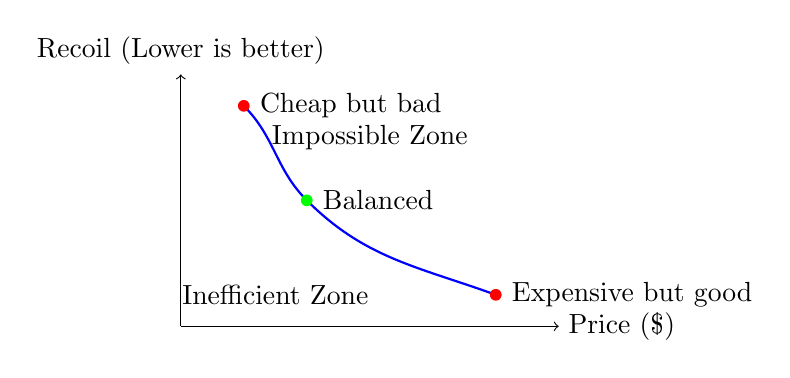
\begin{tikzpicture}[scale=0.8]
        \draw[->] (0,0) -- (6,0) node[right] {Price (\$)};
        \draw[->] (0,0) -- (0,4) node[above] {Recoil (Lower is better)};
        
        \draw[thick, blue] (1, 3.5) to[out=-45, in=135] (2, 2) to[out=-45, in=160] (5, 0.5);
        
        \node[fill=red, circle, inner sep=1.5pt, label=right:Cheap but bad] at (1, 3.5) {};
        \node[fill=green, circle, inner sep=1.5pt, label=right:Balanced] at (2, 2) {};
        \node[fill=red, circle, inner sep=1.5pt, label=right:Expensive but good] at (5, 0.5) {};
        
        \node at (3, 3) {Impossible Zone};
        \node at (1.5, 0.5) {Inefficient Zone};
    \end{tikzpicture}
    \end{center}
    
    \textbf{Why use it?} Allows users to see if spending an extra 50k Roubles actually gives a significant benefit.
\end{frame}

% Slide: Pareto Visualization
\begin{frame}{Pareto Frontier Visualization}
    \begin{center}
        \includegraphics[width=0.9\textwidth,height=0.75\textheight,keepaspectratio]{imgs/page_pareto.png}
    \end{center}
\end{frame}

% Slide: Future Work
\begin{frame}{Future Work & Unimplemented Features}
    \begin{itemize}
        \item \textbf{Hidden Weapon Stats}: Currently unable to retrieve hidden weapon stats, such as recoil angle.
        \item \textbf{Trader Barters}: Currently unable to retrieve trader barter items and their calculated prices.
    \end{itemize}
\end{frame}

% Section 5: Conclusion
\section{Conclusion}

% Acknowledgements
\begin{frame}{Acknowledgements}
    \begin{center}
        \textbf{\Large Data Source}

        \vspace{0.2cm}
        \includegraphics[height=0.9cm]{logos/tarkov-dev-logo.png}

        \vspace{0.1cm}
        Open-source GraphQL API for Escape from Tarkov

        \vspace{0.4cm}
        \textbf{\Large AI Coding Assistants}

        \vspace{0.3cm}
        \begin{tabular}{c @{\hspace{1cm}} c @{\hspace{1cm}} c}
            \includegraphics[height=1.1cm]{logos/claude-color.png} &
            \includegraphics[height=1.1cm]{logos/gemini-color.png} &
            \includegraphics[height=1.1cm]{logos/minimax-color.png} \\[0.2cm]
            \textbf{Claude Code} & \textbf{Gemini CLI} & \textbf{MiniMax} \\[0.1cm]
            Anthropic & Google & MiniMax \\
        \end{tabular}

        \vspace{0.3cm}
        \textit{All the AI assistants helped me with code generation, debugging, and documentation}
    \end{center}
\end{frame}

\end{CJK*}
\end{document}
